%!TEX TS-program = xelatex
%!TEX encoding = UTF-8 Unicode

\documentclass[12pt]{report}
\usepackage{geometry}
\geometry{a4paper}
\usepackage{graphicx}
\usepackage{amssymb}

%\usepackage[numbers]{natbib}

\usepackage{chngcntr}

\usepackage{pst-sigsys}

\usepackage{listings}

\lstset{language=C,
  basicstyle=\footnotesize,
  showspaces=false,
  showstringspaces=false,
  showtabs=false,
  captionpos=b,
  frame=single
  }

%\def\NOHREF{}

\ifdefined\NOHREF
\usepackage{url}
\newcommand{\URL}[1]{\[ \texttt{\emph{#1}} \]}
\newcommand{\href}[2]{#2 (\texttt{\emph{\url{#1}}})} %% not needed probably
\newcommand{\Href}[2]{{#2}} %% fake version for printing
\else
\usepackage{hyperref}
\newcommand{\Href}[2]{\href{#1}{#2}} %% use this for proper href
\newcommand{\URL}[1]{\[ \Href{#1}{\texttt{\emph{#1}}} \]}
\fi

%% use \Href  and for printing we use \cite{something}
%% so we end up with link to the URL and bibliography
%% reference number as well. If \Href is fake there
%% will be no URL in the text.
\newcommand{\AltRef}[3]{\Href{#2}{#1} \cite{#3}}

\usepackage{fontspec,xltxtra,xunicode}
\defaultfontfeatures{Mapping=tex-text}
\setromanfont[Mapping=tex-text]{Hoefler Text}
\setsansfont[Scale=MatchLowercase,Mapping=tex-text]{Gill Sans}
\setmonofont[Scale=MatchLowercase]{Andale Mono}

\title{Digital Reverberator Design in Max/MSP\\using Schroeder Algorithm}
\author{Ilya Dmitrichenko
\\\small DSP Programming Case Study (MU3014C)
\\\small London Metropolitan University}

\date{\today}

\begin{document}
\maketitle
\begingroup
\let\clearpage\relax
\tableofcontents
\listoffigures
\endgroup
\pagebreak

\counterwithout{section}{chapter}

\section{Introduction}

  \subsection{Project Organization}

  As a matter of good practice, a source code revision control system had
  been used in the course of this project. The file format that is used by
  \emph{Max}, is of plain text JSON (JavaScript Object Notation) type, which
  is perfectly suited for use with any revision management system as opposed
  to audio files, which are usually of relatively large size and not very
  much suitable for use with regular version management systems. 

  The revision control tool of choice for this project was \emph{Git}
  \footnote{More information can be found on \emph{Git} homepage:
  \URL{http://git-scm.com/about}}, moreover, in addition to a great set of
  benefits of using \emph{Git} itself, the \emph{GitHub} service enables an
  excellent web integration with a simple user interface. The entire work
  history of this project can be examined on-line:
  \URL{https://github.com/errordeveloper/maxmsp-misc-mu3014c/commits}
  There is no need for the reader to be familiar with how to use \emph{Git},
  since the archive of the current version of the code can be downloaded
  from \emph{GitHub}:
  \URL{https://github.com/errordeveloper/maxmsp-misc-mu3014c/downloads}

  % Further in this report any files will be referenced  ...

  In the project's top-level exists \emph{\texttt{`patchers`}} directory, that
  is where most of the files of interest are located, unless explicitly specified,
  any of file names mentioned in this report can be found there.


  \subsection{Approaches to Reverberator Design}

  Studying the papers which describe various reverberation network topologies,
  it becomes absolutely clear that the degree of experimentation involved in
  the design process is usually very high. According to Jon Dattorro's article
  in the Journal of Audio Engineering Society (1997) \cite{dattorro1997effect},
  where he included a letter from Barry Blesser, who refers to the conversation
  with Manfred Schroeder in the late 1970s where Schroeder have said: \emph{"We
  did the electronic reverberation for amusement because we thought it would be
  fun. Since it took the better part of a day to do 10 seconds of reverberation,
  we only ran one sample of music. The notion of delay time selections was random
  in that we just picked a bunch of numbers and there was no mathematical basis.
  We just wanted to prove it could be done."} Also John Stautner and Miller
  Puckette in their article "Designing Multi-Channel Reverberators" (Computer Music
  Journal, 1982) \cite{puckette1982reverb} point out that \emph{"\dots no attempt
  has been made to imitate the ambience of an existing room or concert hall,
  the methods described herein may lead to such applications when they are
  combined with a consideration of the perceptual importance of attributes of
  the soundfield in a real room."}. Although, the later papers by William Gardner
  \cite{gardner1992virtual, gardner1998algorithms} suggest formulas to calculate
  coefficients, the use of reverberation is not purelly to imitate a specific
  type of room or even an existing room somewhere - it is one of the greates tools
  that musicians can utilies for their artistic expression.



  \subsection{Brief Overview of History of Reverb Topologies}

  Manfred Schroeder had been a pioneer in artificial reverberator design, he
  worked at Bell Laboratories since mid-1950s and published an number of papers
  in the following two decades \cite{dattorro1997effect}. The original
  Schroeder's topology \cite{schroeder1962natural} consisted of 4 parallel comb
  filters generating early echoes and 2 all-pass filters all in series
  \cite{gardner1992virtual}.
  Moorer suggests that Schroeder's design have exhibited fluttering decay
  and poor echo density \cite{moorer1979about}. The fluttering (sometimes also
  called "metallic ringing") can be observed in response to impulsive sounds
  (for example the snare drum), according to Gardner \cite{gardner1992virtual},
  though it is still certainly good for short reverberation times and moderate
  reverberation levels \cite{gardner1998algorithms}. One of the major disadvantages
  is that it \emph{"\dots does not provide a frequency dependent reverberation time"}.
  Moorer \cite{moorer1979about} has modified the comb filter block by adding
  two extra comb filters and a one-pole low-pass filter in the feedback loop
  of each of the comb filters. The low-pass in feedback was intended to
  dump the higher frequencies similarly to how those are absorbed in air.
  Moorer's technique has helped to reduce the unnaturally sounding flutter,
  however it has not eliminated it entirely. There had been a great amount of
  research in this area, where the two biggest problems had been - eliminate
  unnatural colouration and achieve the highest echo density. It should be
  noted that most of the later topologies were designed by modifying the
  feedback path. For example, Puckette and Stautner \cite{puckette1982reverb}
  have achieved much higher echo density in their multi-channel system by
  using a rotation matrix in the feedback loop. Miller Puckette also presents
  this as an example\footnote{It had been a trivial task to implement Puckette's
  reverb in Max and it can be found in the project repository, stored as \texttt{`%
  \href{https://github.com/errordeveloper/maxmsp-misc-mu3014c/blob/master/patchers/reverb.matrix-rotation.maxpat}{reverb.matrix-rotation.maxpat}`}} in his book "The Theory and Technique of Electronic
  Music"\cite{puckette2007theory}.
  Gardner \cite{gardner1998algorithms} also highlighted a number of other
  various feedback loop improvements as well as the work of Jean-Marc Jot in
  early 1990s, who introduced time-varying feedback correcting algorithm,
  which deserves a separate case study and the author of this report certainly
  desires to do so. However, the subject set herein is the earlies reverberator,
  one which Manfred Schroeder has invented in early 1960s.


\section{Implementation}

  \subsection{Building Blocks}
  As mentioned above, the Schroeder's reverb contained 4 parallel comb filters
  in series with 2 all-pass filters, these are also often referred to as the
  \emph{unit reverberators}.

  \subsubsection{Comb Filter}
  The comb filter has a few different uses in audio signal processing (e.g.
  octave doubling \cite{puckette2007theory}) and it seems at first as just
  a simple digital filter. However, instead of delay line being of 1 or 2
  samples in length, it uses a significantly larger length of delay, hence
  exhibits a number of effects, one of which finds the use in reverberation
  network designs.

  Two variants of comb filter design had been encountered in different sources%
  \footnote{For example, Miller Puckette in "Theory and Technique of Electronic
  Music" \cite{puckette2007theory} on page 185 in figure 7.7 gives topology $B$,
  though in the CMJ article \cite{puckette1982reverb} he clearly shows topology
  $A$. While William Gardner \cite{gardner1998algorithms, gardner1992virtual}
  and James Moorer also use $A$, Curtis Roads in "The Computer Music Tutorial"%
  \cite{roads1996computer} on page 479 in fugure 11.79 shows $B$.},
  both appear a little different and it was not very clear at first
  what exactly the difference is (see figures \ref{comb:A} and \ref{comb:B}).
  It is noticeably difficult to implement an arbitrary algorithm using \emph{Max}
  and obtain plain text output which could be copied into a report document,
  hence a small C program was written to simulate impulse response of the two
  topologies and prove that the filters differ very slightly. Code listing
  \ref{comb:test} contains just the functions which implement the algorithms of
  each of the topologies under consideration\footnote{The entire program can be
  view on \emph{GitHub}:
  \URL{https://github.com/errordeveloper/maxmsp-misc-mu3014c/blob/master/tests/comb\_filters.c}}.

  With $g=0.65$ the following output had been obtain for the first 6 samples:
  \begin{verbatim}
  comb_var_a = < 0.000000 1.000000 0.650000 0.422500 0.274625 0.178506 >
  comb_var_b = < 1.000000 0.650000 0.422500 0.274625 0.178506 0.116029 >
  \end{verbatim}
  Hereby it is clear that two of the comb filter variants differ in regards to
  the first sample of the impulse response, the variant $A$ is deduced version of
  $B$ if it have had an additional delay line (as shown in figure \ref{comb:AB}).
  The benefit of using the variant $A$ in reverberator design is due to the fact
  that a number of comb filters will be placed in parallel and will result in an
  undesired effect as show below in terms of difference equations for two comb
  filter with the same input $x_A[n]$ connected in parallel.

  The difference equation for variant $B$ (fig. \ref{comb:B}) of the comb filter
  can be written:\begin{equation}
    y_B[n] = x_B[n] + gy_B[n-m]
  \end{equation}
  For any two different values $m_1$ and $m_2$, and provided that the input
  $x_B[n]$ is a common node, as well as output $y_{B_1}[n]$ and $y_{B_2}[n]$
  are summed in a common node, then the following equation applies:

  \[ y_{B_1}[n] = x_B[n] + gy_{B_1}[n-m_1] \]
  \[ y_{B_2}[n] = x_B[n] + gy_{B_2}[n-m_2] \]
  \[ y_{B_1}[n] + y_{B_2}[n] = 2x_{B}[n] + gy_{B_1}[n-m_1] + gy_{B_2}[n-m_2] \]

  Hence, the output of two parallel comb filters of topology $B$ will contain
  double amplitude of $x_B[n]$, which, in other terms, means that using topology
  $B$ in a reverb will result in undesired contribution to the amount of "dry"
  signal in the output.

  The figure \ref{comb:AB} has been drawn based on empirical results of a
  simulation using the code listed below, however additional proof seems
  necessary.

  \vspace{2em}

\lstset{caption={Extract of the comb filter test program},label=comb:test}
\begin{lstlisting}
void  comb_test_topology_a
 (float y[], float x[], float d, float g) {

  printf("comb_var_a = < ");
  for (int i = 0; i < SIZE; i++) {
  
    y[i] = d;
    d = x[i];
    x[i+1] += d*g;
  
    printf("%f ", y[i]);
  }
  printf(">\n");
}

void  comb_test_topology_b
 (float y[], float x[], float d, float g) {

   printf("comb_var_b = < ");
   for (int i = 0; i < SIZE; i++) {

     d = y[i] = x[i] + g*d;
     printf("%f ", y[i]);
   }
   printf(">\n");
}
\end{lstlisting}

  \begin{figure}
%-- A
\begin{pspicture}[showgrid=false](-9,-1)(6,3)

 \psset{style=RoundCorners,fillstyle=solid,fillcolor=green!14,gratioWh=1.25}

 \psstem[style=Stem,stemtag]{0.000000,1.000000,0.650000,0.422500,0.274625,0.178506}

 %--- Define Blocks:
 \pssignal          (-8,2)     {IA}     {$x_A[n]$}
 \pssignal          (-1,2)     {OA}     {$y_A[n]$}
 \psfblock          (-4,2)     {delA}   {$Z^{-m}$}

 \pscircleop        (-6,2)     {sumA}
 \dotnode           (-3,2)     {dotA}

 \pscircleop  [operation=times](-5.5,0.5){gAd}
 \pssignal          (-5.5,-0.5){gA}      {$g$}
 \ncline{>-}{gA}{gAd}

 %--- Link All Blocks:
 \psset{style=Arrow,fillstyle=none}

 \ncline{->}{IA}{sumA}
 \ncline{->}{sumA}{delA}
 \ncline{->}{delA}{OA}
 \ncangle[angleA=90]{->}{dotA}{gAd}
 \ncangle[angleA=-180,angleB=-135]{->}{gAd}{sumA}

\end{pspicture}
\caption{\emph{Variant A of comb filter and it's impulse response ($m=1$, $g=0.65$)}} \label{comb:A}

\end{figure}

\begin{figure}
%-- B
\begin{pspicture}[showgrid=false](-9,-1)(6,3)

 \psset{style=RoundCorners,fillstyle=solid,fillcolor=green!14,gratioWh=1.25}

 \psstem[style=Stem,stemtag]{1.000000,0.650000,0.422500,0.274625,0.178506,0.116029}
 
 %--- Define Blocks:
 \pssignal          (-8,2)     {IB}     {$x_B[n]$}
 \pssignal          (-1,2)     {OB}     {$y_B[n]$}
 \psfblock          (-4,0.5)   {delB}   {$Z^{-m}$}

 \pscircleop        (-6,2)     {sumB}
 \dotnode           (-3,2)     {dotB}

 \pscircleop  [operation=times](-5.5,0.5){gBd}
 \pssignal          (-5.5,-0.5){gB}      {$g$}
 \ncline{>-}{gB}{gBd}

 %--- Link All Blocks:
 \psset{style=Arrow,fillstyle=none}

 \ncline{->}{IB}{sumB}
 \ncline{->}{sumB}{OB}
 \ncangle{->}{dotB}{delB}
 \ncline{->}{delB}{gBd} \ncangle[angleA=-180,angleB=-145]{->}{gBd}{sumB}

\end{pspicture}
\caption{\emph{Variant B of comb filter and it's impulse response ($m=1$, $g=0.65$)}} \label{comb:B}

\end{figure}


\begin{figure}
%-- B
\begin{pspicture}[showgrid=false](-9,-1)(6,3)

 \psset{style=RoundCorners,fillstyle=solid,fillcolor=green!14,gratioWh=1.25}

 %--- Define Blocks:
 \pssignal          (-8,2)    {IB}     {$x_{AB}[n]$}
 \pssignal          (1,2)     {OB}     {$y_{AB}[n]$}
 \psfblock          (-2,0.5)  {delB}   {$Z^{-m}$}
 \psfblock          (-5.5,2)  {delAB}  {$Z^{-m}$}

 \pscircleop        (-4,2)    {sumB}
 \dotnode           (-1,2)    {dotB}

 \pscircleop  [operation=times](-3.5,0.5){gBd}
 \pssignal          (-3.5,-0.5){gB}      {$g$}
 \ncline{>-}{gB}{gBd}

 %--- Link All Blocks:
 \psset{style=Arrow,fillstyle=none}

 \ncline{->}{IB}{delAB}
 \ncline{->}{sumB}{OB}
 \ncline{->}{delAB}{sumB}
 \ncangle{->}{dotB}{delB}
 \ncline{->}{delB}{gBd}
 \ncangle[angleA=-180,angleB=-145]{->}{gBd}{sumB}

\end{pspicture}
\caption{\emph{Variant B modified to produce direct form of A}} \label{comb:AB}
\end{figure}


  Gardner \cite{gardner1998algorithms} gives the following transfer function
  for the comb filter (variant $A$):\begin{equation}\label{eq:cHAz}
    H_A(z)={{z^{-m}}\over{1-gz^{-m}}}
  \end{equation}
  Given the transfer function (\ref{eq:cHAz}), the difference equation can be
  written in $Z$-domain:\begin{eqnarray}
    Y_A(z)(1-gz^{-m}) &=& X_A(z)(z^{-m})\\
    Y_A(z) &=& X_A(z)(z^{-m}) + Y_A(z)(gz^{-m})
  \end{eqnarray}
  Hence, the time domain difference equation can be derived:
  \begin{equation}\label{eq:cyAn}
    y_A[n] = x_A[n-m] + y_A[n-m]
  \end{equation}
  The equation (\ref{eq:cyAn}) clearly represents the same system which had been
  defined by observation of previous simulation using the C program above.
  The comb filter has it's name because the magnitude response graph, which is
  of comb shape. That is why Schroeder's reverb has the "metallic" sound, it
  is due to additional harmonics introduced by the comb filters. It is also
  important to note that the comb filter is an IIR system and it has multiple
  poles, which are spread harmonically at distance proportional to $m$ modulus
  proportional to $g$. Further analysis of frequency response and it's impact
  on the audible qualities of Schroeder's reverb are outside the scope of this
  report.

  \subsubsection{All-pass Filter}
  As defined by Julius Smith in "Introduction to Digital Filters: With Audio
  Applications" \cite{smith2007introduction}, \emph{"A linear, time-invariant
  filter \dots\ is said to be lossless if it preserves signal energy for every
  input signal"}, which generally implies \begin{equation} \label{eq:allpass}
    H(e^{j\omega})|=1\,\,\forall\omega \end{equation}

  Therefore, by definition, all-pass filter may have any topology provided
  that it's magnitude response is lossless and only it's phase response would
  be of rather more complex nature, though no definition had been made to
  what the phase response should be. Effectively, all-pass filter still
  does affect the audible signal, although only an experienced listener
  could differ the output of an all-pass system from a "dry" input. The
  task herein is to implement Schroeder's reverberator and it's building
  blocks in \emph{Max}, hence only limited number of statements will be made.
  That is said considering how diverse is the field of all-pass filter design,
  since no formal network topology definition exists.

  Looking at Gardner's work \cite{gardner1998algorithms, gardner1992virtual},
  again there appear to be two slightly different implementation of all-pass
  filter, both of which are shown in figures \ref{allpass:A} and \ref{allpass:B}.
  Both of these were also encountered in other literature, including Roads
  \cite{roads1996computer} and Puckette \cite{puckette2007theory}. To compare
  these, it should be sufficient to write down the difference equation for
  each of the variants, using $A$ and $B$ as subscripts for clarity.

  \begin{equation}\label{eq:ayAn}
    y_A[n] = -gx_A[n] +(1-g^2)x_A[n-m] +gy_A[n-m]
  \end{equation}
  \begin{equation}\label{eq:ayBn}
    y_B[n] = -gx_B[n] +x_B[n-m] +gy_B[n-m]
  \end{equation}

  A very similar C program\footnote{Full source code is also available on \emph{GitHub}:
  \URL{https://github.com/errordeveloper/maxmsp-misc-mu3014c/blob/master/tests/allpass\_filters.c}}
  (lis. \ref{allpass:test}) has been written to simulate the behaviour for two all-pass
  filter implementations (fig. \ref{allpass:A} \& \ref{allpass:B}). Unlike the program
  in listing \ref{comb:test}, this was rather much simpler to implement since
  the difference equation was known already\footnote{It was somewhat more
  difficult to write the equation for the comb filters, since the diagrams
  look very different to a common $n$-pole/$n$-zero filter.}. It helped,
  however, to obtain the impulse response for each of the variants which is
  show below for the first 6 sample with $g=0.5$ and $m=1$. It should be also
  noted that the value of $m$ will affect the frequency response of the filter
  and it's impulse response, nevertheless setting $m=1$ in this simulation
  does give a good picture where the difference between two topologies can be
  observer. Namely, the data shown below confirms that the extra multiply node
  on the diagram only affect the decay curve of the impulse response.
  \begin{verbatim}
  allpass_var_a = < -0.500000 0.500000 0.250000 0.125000 0.062500 0.031250 >
  allpass_var_b = < -0.500000 0.750000 0.375000 0.187500 0.093750 0.046875 >
  \end{verbatim}
  As it has been said already, the objection of this report is rather more
  practical, hence there is no detailed derivation of $H(z)$ and proof of
  that equation \ref{eq:allpass} is true for the above all-pass filters,
  in fact that would be rather redundant.
  \pagebreak
\lstset{caption={Extract of the all-pass filter test program},label=allpass:test}
\begin{lstlisting}
void  allpass_test_topology_a
 (float y[], float x[], float d, float g) {

  printf("allpass_var_a = < ");
  for (int i = 0; i < SIZE; i++) {
  
    if (i == 0) { 
      y[i] = -g*x[i];
    } else {
      y[i] = -g*x[i]+(1-g*g)*x[i-1]+g*y[i-1];
    }
    printf("%f ", y[i]);
  }
  printf(">\n");
}

void  allpass_test_topology_b
 (float y[], float x[], float d, float g) {
   printf("allpass_var_b = < ");
   for (int i = 0; i < SIZE; i++) {

     if (i == 0) { 
       y[i] = -g*x[i];
     } else {
       y[i] = -g*x[i]+x[i-1]+g*y[i-1];
     }
     printf("%f ", y[i]);
   }
   printf(">\n");
}
\end{lstlisting}
\pagebreak
\begin{figure} \begin{pspicture}[showgrid=true](-5,-1)(5,5)

 \psset{style=RoundCorners,fillstyle=solid,fillcolor=green!14,gratioWh=1.25}


 %--- Define Blocks:

 \pssignal          (-4,2.5)    {I}     {$x[n]$}
 \pssignal          (4.5,2.5)   {O}     {$y[n]$}

 \dotnode           (-3,2.5)    {dot0}
 \pscircleop        (-2,2.5)    {sum0}

 \dotnode           (1,2.5)     {dot1}
 \pscircleop        (3,2.5)     {sum1}


 \psfblock          (-0.5,2.5)  {del}   {$Z^{-m}$}


 \pscircleop  [operation=times](-1,1){g0d}
 \pssignal          (-1,0)      {g0}    {$-g$}
 \ncline{>-}{g0}{g0d}

 \pscircleop  [operation=times](0,4){g1d}
 \pssignal          (0,5)    {g1}    {$g$}
 \ncline{>-}{g1}{g1d}

 \pscircleop[operation=times](2,2.5){g2d}
 \pssignal          (2,1.5)    {g2}    {$1-g^2$}
 \ncline{>-}{g2}{g2d}


 %--- Link All Blocks:

 \psset{style=Arrow,fillstyle=none}

 \ncline{->}{I}{sum0}
 \ncline{->}{sum0}{del}
 \ncline{->}{del}{g2d}
 \ncline{->}{g2d}{sum1}
 \ncline{->}{sum1}{O}

 \ncangle[angleA=-90,angleB=180]{->}{dot0}{g0d}
 \ncangle[angleB=-45]{->}{g0d}{sum1}
 \ncangle[angleA=90]{->}{dot1}{g1d}
 \ncangle[angleA=180,angleB=145]{->}{g1d}{sum0}


\end{pspicture} \caption{\emph {All-pass Filter}} \label{allpass:A}\end{figure}

\begin{figure} \begin{pspicture}[showgrid=false](-5,0)(5,6)

 \psset{style=RoundCorners,fillstyle=solid,fillcolor=green!14,gratioWh=1.25}


 %--- Define Blocks:

 \pssignal          (-4,3.5)    {I}     {$x[n]$}
 \pssignal          (4,3.5)     {O}     {$y[n]$}

 \dotnode           (-2.5,3.5)    {dot0}
 \pscircleop        (-1.5,3.5)    {sum0}

 \psfblock          (0,3.5)       {del}   {$Z^{-m}$}

 \pscircleop        (1.5,3.5)     {sum1}
 \dotnode           (2.5,3.5)     {dot1}



 \pscircleop  [operation=times](0.5,5){g0d}
 \pssignal          (0.5,6)    {g0}    {$g$}
 \ncline{>-}{g0}{g0d}

 \pscircleop  [operation=times](-0.5,2){g1d}
 \pssignal          (-0.5,1)    {g1}    {$-g$}
 \ncline{>-}{g1}{g1d}


 %--- Link All Blocks:

 \psset{style=Arrow,fillstyle=none}

 \ncline{->}{I}{sum0}
 \ncline{->}{sum0}{del}
 \ncline{->}{del}{sum1}
 \ncline{->}{sum1}{O}

 \ncangle[angleA=-90]{->}{dot1}{g0d}
 \ncangle[angleA=-180,angleB=-90]{->}{g1d}{dot0}
 %\ncangle[angleA=-180,angleB=-90]{<-}{g1d}{dot0}
 \ncangle[angleA=-180,angleB=145]{->}{g0d}{sum0}
 \ncangle[angleB=-45]{->}{g1d}{sum1}


\end{pspicture} \caption{\emph {All-pass Filter}} \label{allpass:B}\end{figure}


\subsection{Max/MSP Patches}

The implementation of Schroeder's reverberator requires two major components -
a comb and an all-pass filter. \emph{Max/MSP} provides built-in objects for
these two types of filters, however the task of this project had been to
implement the reverberator utilising only the most primitive of instances of
built-in objects. Figures \ref{max:comb} and \ref{max:allpass} demonstrate
the unit reverberators which had been implemented and figure \ref{max:guts}
show the inner body of the patch filed as
\emph{\texttt{`reverb.schroeder\~{}.maxpat`}}.

Once the reverberator has been implemented, the major challenge was to find
the appropriate ratio of the gain and delay values. According to Gardner
\cite{gardner1998algorithms}, the following formula can be used to find the
values of $g_i$ from $m_i$:\begin{equation}\label{eq:coef}
  g_i=10^{-3m_i/T_r}
\end{equation}
where $m_i$ is the delay time in seconds and $T_r$ is the reverberation time.
The implementation in \emph{Max} (shown in figure \ref{max:guts}) would had
been rather unacceptable without this particular relation, because the lister
may simply damaged their ears. The sub-patch \emph{\texttt{`calc.coef`}}
implements the equation given by Gardner, there are also \emph{\texttt{`filt.comb-lp\~{}`}} and
\emph{\texttt{`filt.allpass-time-delay\~{}`}} which are representing the comb
filter with low-pass feedback (Moorer's comb) and an all-pass filter as seen
in figure \ref{allpass:A}\ . The reason why the low-pass filter had to be
placed in the feedback loop of the comb filter, is simply because the sound
without it was rather hard to believe being of a reverb unit. It is very clear
that a commercially available reverberator today sounds much different from
it's "early digital" ancestor circa 1960s, moreover it becomes obvious what
sort of "metallic" and "unnatural" sounds were described by all of the
researchers cited.


The source code repository of this project (see sec. 1.1) also contains
several files which are the results of some of the early experiments.
Amongst miscellaneous, there is a implementation of Puckette \& Stautner
rotation-matrix stereo reverb (filename \emph{\texttt{`reverb.matrix-rotation.maxpat`}})
as well as some more primitive filters (e.g. \emph{\texttt{`filt.1st-order\~{}.maxpat`}}
and \emph{\texttt{`filt.2nd-order\~{}.maxpat`}}).

\begin{figure}
  \centering
  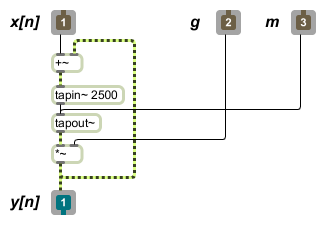
\includegraphics[scale=0.5]{images/filt.comb.png}
  \caption{\emph{Comb filter implemented in Max/MSP}}
  \label{max:comb}
\end{figure}
\begin{figure}
  \centering
  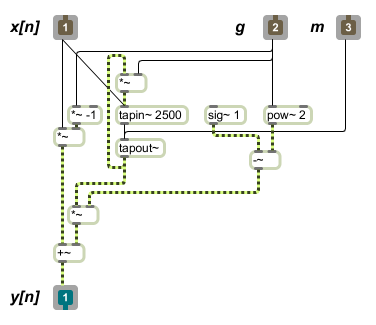
\includegraphics[scale=0.5]{images/filt.allpass.png}
  \caption{\emph{All-pass filter implemented in Max/MSP}}
  \label{max:allpass}
\end{figure}
\begin{figure}
  \centering
  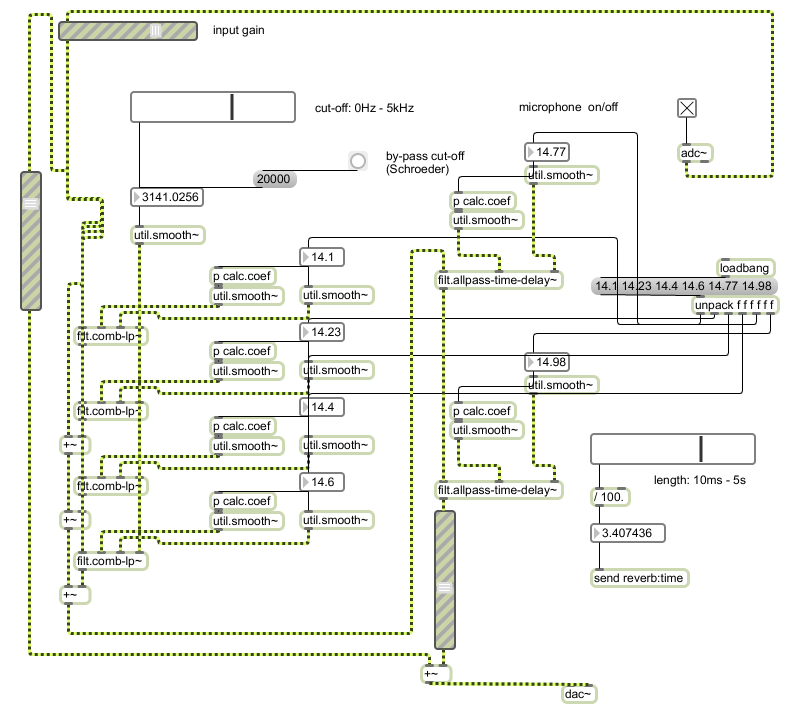
\includegraphics[scale=0.5]{images/guts.png}
  \caption{\emph{Internals of the reverberator patch}}
  \label{max:guts}
\end{figure}



%%%%%%%%%%%%%%%%%%%%%%%%%%%%%%%%%%%%%%%%%%%%%%%%%%%%%%%%%%%%%%%%%%%%%%%%

\bibliographystyle{acm}
%\bibliographystyle{agsm}
%\bibliographystyle{plainnat}

\bibliography{MU3014C_coursework}

\end{document}  
